\documentclass[10pt,journal,compsoc]{IEEEtran}
\usepackage[T1]{fontenc}
\usepackage[utf8]{inputenc}
\usepackage{microtype}
\usepackage{amsmath,amssymb,amsfonts,amsthm}
\usepackage{booktabs}
\usepackage{graphicx}
\usepackage{adjustbox}
\usepackage{placeins}
\usepackage{multirow}
\usepackage{array}
\usepackage{url}
\usepackage[hidelinks]{hyperref}

\Urlmuskip=0mu plus 2mu\relax
\emergencystretch=1.6em
\extrafloats{48}
\newtheorem{proposition}{Proposition}

\begin{document}

\title{CAPQ-Pareto: Coordinate-Confidential Post-Quantum Hybrid Vector-Relational Cloud Querying via Session Pooling, Single-Ciphertext CKKS Aggregation, and Lagged Contextual Control}

\author{Preecha~Noiumkar,~\IEEEmembership{Member,~IEEE}%
\thanks{P.~Noiumkar is with the Department of Information Technology, Faculty of Informatics, Mahasarakham University, Maha Sarakham 44150, Thailand (e-mail: preecha.n@msu.ac.th; ORCID: 0009-0000-5964-4896).}%
\thanks{This research project was financially supported by the Faculty of Informatics, Mahasarakham University. Electronic Supplementary Material and reproducible benchmark artifacts (28 verified files with SHA-256 provenance manifests) accompany this submission.}}

\IEEEtitleabstractindextext{%
\begin{abstract}
Migrating hybrid relational-vector cloud databases to post-quantum cryptography (PQC) while protecting query coordinates introduces compounding network and homomorphic overheads: per-query hybrid \texttt{X25519+ML-KEM-768} and \texttt{ML-DSA-65} handshakes add 14.67~KB, whereas multi-ciphertext \texttt{RNS-CKKS} Approximate Nearest Neighbor (ANN) responses inflate wire payloads. We present \textbf{CAPQ-Pareto}, combining persistent hybrid PQC session pooling, single-MTU asymmetric \texttt{INT8} quantization, boundary-replicated \texttt{SPANN-CKKS} with server-side single-ciphertext (1-CT) slot aggregation, and a lagged five-dimensional discounted linear contextual bandit (\texttt{D-LinUCB}). Across 1,440 live three-region Google Cloud Wide-Area Network (WAN) queries and 2,304 controlled queries against a fair static \texttt{QUIC+INT8+SPANN+1-CT} baseline (\texttt{M8}), we establish three bounded findings. First, session pooling and single-MTU \texttt{INT8} drive primary latency gains, cutting live mean latency by 61.9\% in Bangkok (126.89 to 48.35~ms, $p < 0.0001$) and 70.9\% in Singapore (266.33 to 77.63~ms, $p < 0.0001$). Second, $N=8192$ 1-CT aggregation shrinks confidential responses $7.05\times$ (909.3 to 129.0~KB) and decryption from 3.28 to 0.59~ms across 500 SIFT-1M queries, though fixed-budget ($M=224$) Recall@10 declines from 0.7882 (5k) to 0.6364 (25k) and 0.5502 (100k; 0.7322 at $M=512$). Third, under full 5D context, \texttt{D-LinUCB} ($\gamma=0.88, \nu=0.06, \lambda=0.08$) matches \texttt{M8} on unimpaired paths ($p = 0.262$) while restoring SLA compliance from 57.81\% to 92.69\% during RFC~9308 UDP-policing inversions ($p = 0.0059$).
\end{abstract}

\begin{IEEEkeywords}
Post-quantum cryptography, ML-KEM, ML-DSA, RNS-CKKS homomorphic encryption, vector databases, pgvector HNSW, QUIC transport, non-stationary contextual bandits, cloud performance evaluation.
\end{IEEEkeywords}}

\maketitle
\IEEEdisplaynontitleabstractindextext
\IEEEpeerreviewmaketitle

\section{Introduction}
Modern enterprise retrieval-augmented generation (RAG) and transactional analytics consolidate relational predicates, JSON metadata filters, and dense vector similarity search within unified cloud data engines~\cite{wang2021milvus,malkov2018hnsw}. Transitioning client-to-cloud database links to NIST-standardized post-quantum cryptography---specifically FIPS~203 \texttt{ML-KEM}~\cite{fips203} and FIPS~204 \texttt{ML-DSA}~\cite{fips204}---while simultaneously protecting sensitive query embeddings against untrusted cloud operators exposes three interacting systems challenges:

\begin{enumerate}
\item \textbf{PQC Handshake Amplification vs.\ Transport Head-of-Line Blocking:} While C-level \texttt{liboqs}~\cite{stebila2016liboqs} cryptographic execution for \texttt{ML-KEM-768} key encapsulation (0.024~ms) and three-certificate \texttt{ML-DSA-65} verification (0.085~ms) is sub-millisecond on modern processors, a full hybrid TLS~1.3 handshake transmits 14,665~B (exceeding ten 1,500-B Ethernet MTU frames)~\cite{paquin2020pqctls,sikeridis2020pqtls}. Even with TLS certificate compression (RFC~8879)~\cite{rfc8879}, which shrinks redundant X.509 ASN.1 metadata by roughly 15--22\% while leaving high-entropy lattice keys and signatures incompressible, unamortized handshakes incur multi-RTT congestion windows over regional and transcontinental WANs.
\item \textbf{Wire Inflation and Recall Degradation in Homomorphic ANN:} Evaluating inner products under approximate homomorphic encryption (\texttt{RNS-CKKS}~\cite{cheon2017ckks,albadawi2022openfhe}) hides plaintext query coordinates from the cloud server (which we strictly term \emph{coordinate-confidential} search, as public centroid routing metadata remains client-visible and server-indexed~\cite{henzinger2023tiptoe}). However, returning separate ciphertexts per SIMD batch (\texttt{Multi-CT}, 909.3~KB for 14 blocks on $N=4096$) triggers severe TCP retransmission stalls under modest WAN packet loss. Conversely, constant-time bucket evaluation exhibits a fundamental recall-versus-corpus-size trade-off as enclave cardinality grows from $5\times 10^3$ to $10^5$ vectors.
\item \textbf{Disentangling Static Systems Engineering from Online Bandit Adaptation:} Prior adaptive cloud transport controllers often compare online learners against weak baselines that lack static wire optimizations. To isolate genuine online learning gains from static engineering, an adaptive controller must be benchmarked directly against a fair static baseline equipped with identical session pooling, quantization, \texttt{SPANN} boundary replication~\cite{chen2021spann}, and single-ciphertext aggregation.
\end{enumerate}

\begin{figure*}[!t]
\centering
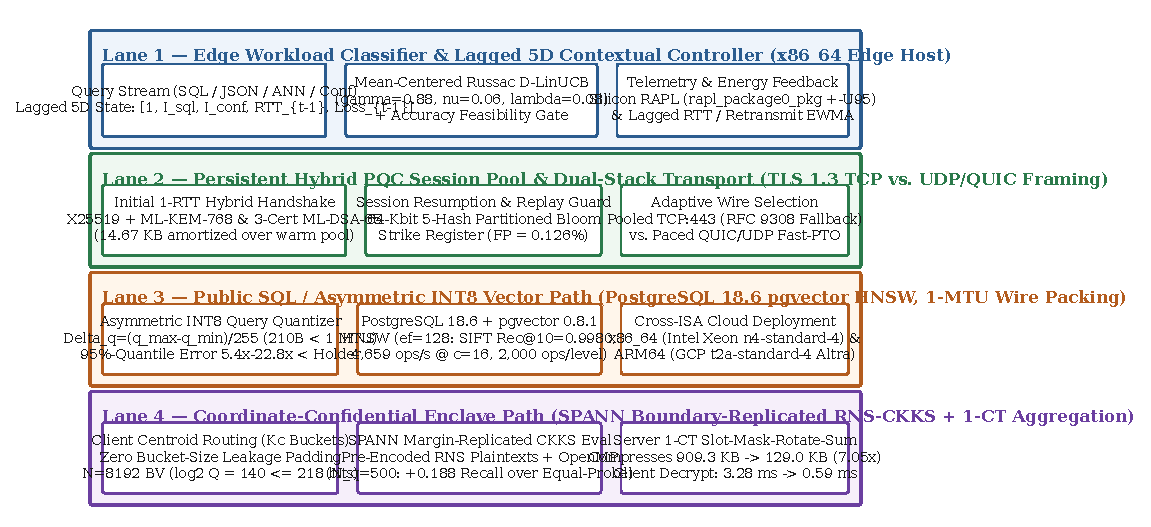
\includegraphics[width=0.98\textwidth]{figures/fig1_architecture.pdf}
\caption{CAPQ-Pareto four-swimlane campus/fiber-to-cloud architecture integrating a lagged 5D contextual controller, persistent hybrid PQC session pooling with a 64-Kbit Bloom strike register, single-MTU asymmetric \texttt{INT8} public vector querying on PostgreSQL~18.6 \texttt{pgvector} HNSW, and coordinate-confidential \texttt{SPANN-CKKS} evaluation with $N=8192$ server-side 1-CT slot aggregation across x86\_64 (\texttt{n4-standard-4}) and ARM64 (\texttt{t2a-standard-4} Ampere Altra Neoverse-N1) cloud nodes.}
\label{fig:arch}
\end{figure*}

\subsection{Contributions and Empirical Scope}
This paper presents a transparent empirical and methodological study of \textbf{CAPQ-Pareto} (Fig.~\ref{fig:arch}), backed by 28 reproducible artifacts (14 raw/summary datasets and 14 vector figures; Table~\ref{tab:taxonomy}):
\begin{itemize}
\item \textbf{Transport Stack and Asymmetric INT8 Concentration Analysis:} We implement persistent hybrid \texttt{X25519+ML-KEM-768} session pooling over TLS~1.3/TCP and \texttt{aioquic}~1.2.0/UDP framing with a 64-Kbit 5-hash partitioned Bloom replay register (exact theoretical false-positive probability 0.126\%). In Proposition~\ref{prop:int8}, we formalize the distinction between corpus-distribution randomness $\mathcal{P}(\mathbf{q},\mathbf{x})$ for deterministic rounding and conditional rounding noise $\mathbb{P}(\boldsymbol{\xi}\mid\mathbf{q},\mathbf{x})$ for unbiased stochastic rounding, demonstrating across 10,000 real SIFT-1M and BGE-M3 pairs that at the matched 95\% quantile, sub-Gaussian error is 5.39$\times$ ($D=128$) and 22.76$\times$ ($D=1024$) tighter than worst-case H\"older bounds.
\item \textbf{True 1-CT RNS-CKKS Aggregation and Controlled Equal-Budget Audit:} Using a native C++ \texttt{OpenFHE}~\cite{albadawi2022openfhe} bridge under strict \texttt{HEStd\_128\_classic} security, we show why depth-2 slot-masking overflows $N=4096$ ($\log_2 Q \le 109$~bits) and implement depth-2 1-CT slot-mask-rotate-sum aggregation on $N=8192$ ($\log_2 Q = 140 \le 218$~bits). Across $N_q = 500$ queries, 1-CT reduces response wire size from 909.3~KB to 129.0~KB and client decryption from 3.28 to 0.59~ms at the cost of +16.10~ms server homomorphic masking/rotation. We report full Recall@10 confidence intervals under both equal-probe ($r=2$) and equal-candidate-budget ($M=224$) controls at $K_c \in \{96, 192\}$ and across enclave sizes $N \in \{5\text{k}, 25\text{k}, 100\text{k}\}$.
\item \textbf{Fair Baseline Separation (\texttt{M8}) and Two-Track WAN Evaluation:} We introduce \texttt{M8} (\texttt{Static Pooled QUIC + INT8 + SPANN + 1-CT}) alongside legacy \texttt{M7} (\texttt{Pooled TCP + FP32 + SPANN + Multi-CT}). Using a frozen hyperparameter configuration ($\gamma=0.88, \nu=0.06, \lambda=0.08$), $2^5$ factorial GLM with 10,000 within-block permutations, silicon RAPL (\nolinkurl{rapl_package0_pkg}) ISO GUM $\pm U_{95}$ energy metrology~\cite{khan2018rapl,iso_gum_2008}, a pure 1,440-query live 3-region GCP campaign (\texttt{M1--M5}), and a 2,304-query controlled 3-region \texttt{netns} campaign (\texttt{M1--M8}), we delineate where static engineering suffices and where online adaptation prevents SLA collapse.
\end{itemize}

\begin{table*}[!t]
\centering
\caption{Architectural Taxonomy of Evaluated System Modes (\texttt{M1--M8}) Separating Static Wire/Cryptographic Gains from Online Adaptation}
\label{tab:taxonomy}
\footnotesize
\begin{adjustbox}{max width=\textwidth}
\begin{tabular}{lllllllc}
\toprule
\textbf{Mode} & \textbf{Session \& Key Exch.} & \textbf{Wire Transport} & \textbf{Public Vec.} & \textbf{Conf.\ Index} & \textbf{CKKS Return} & \textbf{Controller} & \textbf{Coord.-Conf.} \\
\midrule
\texttt{M1} & Fresh Hybrid PQC / query & TCP TLS~1.3 & FP32 (512~B) & SPANN ($r=2$) & Multi-CT (909~KB) & Static & Yes \\
\texttt{M2} & Fresh Classical TLS~1.3 & TCP TLS~1.3 & FP32 (512~B) & Plaintext HNSW & Plaintext (0~KB CT) & Static & No \\
\texttt{M3} & Warm Classical Pool & TCP TLS~1.3 & FP32 (512~B) & Plaintext / 1-Probe & Plaintext / 1-Probe & Static & No / Partial \\
\texttt{M4} & Warm Hybrid PQC Pool & TCP TLS~1.3 & INT8 / FP32 & Disjoint ($r=1$) & 1-CT (129~KB) & Static Heuristic & Yes (Low Rec.) \\
\texttt{M6} & Warm Hybrid PQC Pool & TCP TLS~1.3 & FP32 (512~B) & Disjoint ($r=2$) & 1-CT (129~KB) & Static & Yes \\
\texttt{M7} & Warm Hybrid PQC Pool & TCP TLS~1.3 & FP32 (512~B) & SPANN ($r=2$) & Multi-CT (909~KB) & Static & Yes \\
\texttt{M8} \textbf{(Fair Static)} & Warm Hybrid PQC Pool & Paced QUIC/UDP & Asym.\ INT8 & SPANN ($r=2$) & \textbf{True 1-CT (129~KB)} & \textbf{Static Fixed} & \textbf{Yes} \\
\texttt{M5} \textbf{(CAPQ-Pareto)} & Warm Hybrid PQC Pool & Dual TCP / QUIC & Asym.\ INT8 & SPANN ($r=2$) & \textbf{True 1-CT (129~KB)} & \textbf{5D D-LinUCB} & \textbf{Yes} \\
\bottomrule
\end{tabular}
\end{adjustbox}
\end{table*}

\section{System Model, Threat Model, and Transport Stack}
\subsection{Coordinate-Confidential Threat Model}
We consider an edge gateway located on a campus/fiber-to-cloud enterprise network issuing a mixed stream of transactional SQL point lookups (25\%), public ANN vector queries (50\%), and confidential vector queries (25\%) to an untrusted cloud server. Network links are exposed to store-now-decrypt-later adversaries, motivating hybrid \texttt{X25519+ML-KEM-768} key exchange and \texttt{ML-DSA-65} authentication~\cite{fips203,fips204}. For the 25\% confidential query class, the cloud server is modeled as honest-but-curious: the client stores a lightweight float32 table of $K_c$ public cluster centroids ($K_c \times 128 \times 4$~B $= 48$~KB at $K_c=96$, or $640$~KB at $K_c=1280$), selects the $r$ nearest bucket IDs locally, and transmits the bucket IDs alongside an \texttt{RNS-CKKS} ciphertext encrypting the query vector $\mathbf{q} \in \mathbb{S}^{d-1}$.

Crucially, we avoid overclaiming ``zero-trust'' obliviousness: like cluster-routed private search systems such as Tiptoe~\cite{henzinger2023tiptoe}, coarse bucket IDs are visible to the server, whereas fine-grained vector coordinates within probed regions remain computationally indistinguishable under Ring-LWE (\texttt{HEStd\_128\_classic}). To eliminate secondary side channels from variable cluster cardinalities, every \texttt{SPANN} bucket on the server is padded with zero-vector dummy slots to an identical constant $B_{\max}$, ensuring zero mutual information $I(S; |B_k|) = 0$~bits between execution trace $S$ and true cluster population $|B_k|$~\cite{paninski2003entropy}.

\subsection{QUIC Transport Implementation and Hybrid PQC 0-RTT Security Semantics}
Our control and data planes operate over OpenSSL~3.5.5 paired with C \texttt{liboqs} (\texttt{ML-KEM-768} + \texttt{ML-DSA-65}) for initial 1-RTT hybrid session establishment, and Python \texttt{aioquic}~1.2.0 / paced UDP framing (1,350-B maximum datagram payload per RFC~9000~\cite{rfc9000}, selective missing-frame recovery per RFC~9002~\cite{rfc9002}) for connection-pooled low-latency transport. Our three-certificate PKI chain transmits one intermediate CA \texttt{ML-DSA-65} public key ($1,952$~B; root CA pinned in client trust store) plus three \texttt{ML-DSA-65} signatures ($3 \times 3,309 = 9,927$~B, totaling $11,879$~B for chain material, or $13,831$~B if leaf PK is counted separately, and $14,665$~B total hybrid handshake flight including \texttt{X25519+ML-KEM-768} shares and TLS framing).

A critical cryptographic distinction governs QUIC 0-RTT early data: 0-RTT resumption encrypts early frames under a Pre-Shared Key (PSK) resumption secret derived from the preceding 1-RTT hybrid \texttt{X25519+ML-KEM-768} handshake. While this PSK inherits post-quantum resistance against passive capture provided session ticket keys remain secret, \emph{0-RTT early data lacks per-query forward secrecy if the server's session-ticket encryption key (STEK) is subsequently compromised, and is inherently vulnerable to network replay}~\cite{rfc9000}. Accordingly, CAPQ-Pareto enforces two strict protocol guards: (i)~0-RTT framing is restricted exclusively to idempotent read-only vector/SQL queries (never state-mutating writes), and (ii)~the cloud ingress enforces single-use nonces via an in-memory 64-Kbit ($m = 65,536$~bits) 5-hash ($k=5$) partitioned Bloom strike register rotated every epoch of $n = 4,000$ tickets, yielding an exact combinatorial false-positive rate of:
\begin{equation}
p_{\text{FP}} = \left(1 - \left(1 - \frac{1}{m}\right)^{kn}\right)^k = 0.001258 \approx 0.126\%,
\end{equation}
which triggers a transparent 1-RTT fallback on collision with zero query-drop error.

\section{Public Tier: Asymmetric INT8 Bounds and PG18.6 HNSW}
\subsection{Sub-Gaussian Concentration and Probability Spaces}
For public ANN queries ($\mathbf{q}, \mathbf{x} \in \mathbb{S}^{D-1}$), transmitting 32-bit floats requires $4D$~B ($4,096$~B at $D=1024$, spanning three TCP/QUIC segments). Asymmetric per-query \texttt{INT8} quantization maps $q_i \mapsto \hat{q}_i$ using step size $\Delta_q = (q_{\max} - q_{\min})/255$, shrinking $D=128$ queries to $\approx 210$~B (including headers) and $D=1024$ queries to $1,032$~B (fitting comfortably inside a single 1,500-B MTU frame).

\begin{proposition}[Asymmetric INT8 Inner-Product Error Under Distinct Rounding Spaces]\label{prop:int8}
Let $\mathbf{q}, \mathbf{x} \in \mathbb{S}^{D-1}$ with step size $\Delta_q = (q_{\max} - q_{\min})/255$ and error $\varepsilon(\mathbf{q},\mathbf{x}) = \langle \hat{\mathbf{q}} - \mathbf{q}, \mathbf{x} \rangle = \sum_{i=1}^D e_i x_i$, where $|e_i| \le \Delta_q / 2$.
\begin{enumerate}
\item \textbf{Deterministic Worst-Case Bound:} By H\"older's inequality, $|\varepsilon(\mathbf{q},\mathbf{x})| \le \frac{1}{2}\Delta_q \|\mathbf{x}\|_1 \le \frac{1}{2}\Delta_q \sqrt{D}$ with probability~1.
\item \textbf{Stochastic Unbiased Rounding ($\mathbb{P}_{\boldsymbol{\xi}\mid\mathbf{q},\mathbf{x}}$):} Under randomized unbiased rounding $\hat{q}_i = q_{\min} + \Delta_q(\lfloor u_i \rfloor + \xi_i)$ with independent $\xi_i \sim \mathrm{Bernoulli}(u_i - \lfloor u_i \rfloor)$ conditioned on fixed $(\mathbf{q},\mathbf{x})$, $\mathbb{E}_{\boldsymbol{\xi}}[\varepsilon \mid \mathbf{q},\mathbf{x}] = 0$, $\mathrm{Var}_{\boldsymbol{\xi}}(\varepsilon \mid \mathbf{q},\mathbf{x}) \le \Delta_q^2 / 6$, and Hoeffding's inequality yields a conservative distribution-free finite-sample $1-\zeta$ bound:
\begin{equation}
\mathbb{P}_{\boldsymbol{\xi}}\!\left(|\varepsilon| \le \Delta_q \sqrt{\tfrac{1}{2}\ln(2/\zeta)} \,\middle|\, \mathbf{q},\mathbf{x}\right) \ge 1 - \zeta.
\end{equation}
\item \textbf{Deterministic Nearest Rounding ($\mathcal{P}_{\mathcal{Q}\times\mathcal{D}}$):} When $\hat{q}_i = q_{\min} + \Delta_q \mathrm{round}(u_i)$, no randomness remains once $(\mathbf{q},\mathbf{x})$ is fixed. Over random query-document pairs $(\mathbf{q},\mathbf{x}) \sim \mathcal{P}_{\mathcal{Q}\times\mathcal{D}}$ whose scaled residuals are asymptotically uniform on $[-\Delta_q/2, \Delta_q/2]$ and weakly dependent across coordinates, $\sigma_{\text{det}} \approx \mathbb{E}[\Delta_q]/\sqrt{12}$, yielding a 95\% central limit half-width of $1.96\,\sigma_{\text{emp}}$.
\end{enumerate}
\end{proposition}

\begin{figure}[!t]
\centering
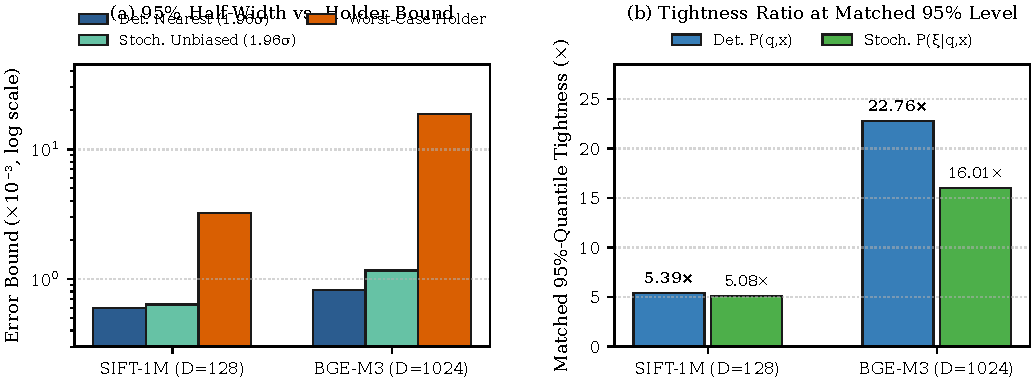
\includegraphics[width=\columnwidth]{figures/fig2_prop1_same_quantile95.pdf}
\caption{Proposition~\ref{prop:int8} audit across 10,000 real query-vector pairs on SIFT-1M ($D=128$) and BGE-M3 ($D=1024$): (a)~95\% half-width ($1.96\sigma_{\text{emp}}$) versus worst-case H\"older bound; (b)~tightness ratio evaluated fairly at the matched 95\% quantile.}
\label{fig:prop1}
\end{figure}

\begin{table}[!t]
\centering
\caption{PostgreSQL~18.6 (\texttt{pgvector}~0.8.1) HNSW \texttt{ef\_search} Sweep ($N=300$) and Concurrency Scaling (2,000 SQL Ops/Level)}
\label{tab:hnsw}
\footnotesize
\setlength{\tabcolsep}{3.5pt}
\begin{adjustbox}{max width=\columnwidth}
\begin{tabular}{lrrrrr}
\toprule
\multicolumn{6}{c}{\textbf{Part A: HNSW \texttt{ef\_search} Recall-Latency ($m=16, \text{ef\_c}=64$)}} \\
\textbf{Corpus} & \textbf{\texttt{ef}} & \textbf{Queries} & \textbf{Rec@10} & \textbf{p50 (ms)} & \textbf{p95 (ms)} \\
\midrule
SIFT-50k (128d) & 32 & 300 & 0.9730 & 0.58 & 0.72 \\
SIFT-50k (128d) & 64 & 300 & 0.9927 & 0.81 & 1.03 \\
SIFT-50k (128d) & 128 & 300 & 0.9980 & 1.07 & 1.34 \\
SIFT-50k (128d) & 256 & 300 & 0.9990 & 1.68 & 2.11 \\
BGE-25k (1024d) & 32 & 300 & 0.8237 & 0.66 & 0.95 \\
BGE-25k (1024d) & 64 & 300 & 0.9083 & 0.88 & 1.28 \\
BGE-25k (1024d) & 128 & 300 & 0.9563 & 1.29 & 1.85 \\
BGE-25k (1024d) & 256 & 300 & 0.9880 & 2.16 & 3.36 \\
\midrule
\multicolumn{6}{c}{\textbf{Part B: Concurrency Scaling (\texttt{ef}=128, 10,000 Total SQL Ops)}} \\
\textbf{Workload} & \textbf{Ops} & \textbf{Ops/s} & \textbf{p50 (ms)} & \textbf{p95 (ms)} & \textbf{p99 (ms)} \\
\midrule
SIFT-50k ($c=1$) & 2000 & 990.3 & 0.98 & 1.21 & 1.42 \\
SIFT-50k ($c=4$) & 2000 & 3125.4 & 1.10 & 1.38 & 1.52 \\
SIFT-50k ($c=8$) & 2000 & 4524.3 & 1.34 & 1.75 & 2.03 \\
SIFT-50k ($c=16$) & 2000 & 4659.3 & 2.31 & 3.38 & 3.85 \\
SIFT-50k ($c=32$) & 2000 & 3973.5 & 4.53 & 7.90 & 10.00 \\
\bottomrule
\end{tabular}
\end{adjustbox}
\end{table}

\begin{table*}[!t]
\centering
\caption{Empirical Verification of Proposition~\ref{prop:int8} Across 10,000 Real Pairs Comparing Matched 95\% Quantiles ($1.96\sigma_{\text{emp}}$ and Empirical $q_{95}$) Against Worst-Case H\"older Bounds}
\label{tab:prop1}
\footnotesize
\begin{adjustbox}{max width=\textwidth}
\begin{tabular}{llrrrrrr}
\toprule
\textbf{Corpus} & \textbf{Rounding \& Probability Space} & \textbf{Theo.\ $\sigma$} & \textbf{Emp.\ $\sigma$} & \textbf{Emp.\ $|e|_{95\%}$} & \textbf{$1.96\sigma_{\text{emp}}$} & \textbf{Worst-Case H\"older} & \textbf{Matched 95\% Tightness} \\
\midrule
SIFT1M-128d ($D=128$) & Deterministic Nearest $\mathcal{P}_{\mathcal{Q}\times\mathcal{D}}(\mathbf{q},\mathbf{x})$ & 0.000277 & 0.000306 & 0.000594 & 0.000599 & 0.003228 & \textbf{5.39$\times$} \\
SIFT1M-128d ($D=128$) & Stochastic Unbiased $\mathbb{P}_{\boldsymbol{\xi}\mid\mathbf{q},\mathbf{x}}(\cdot\mid\mathbf{q},\mathbf{x})$ & 0.000392 & 0.000324 & 0.000642 & 0.000635 & 0.003228 & \textbf{5.08$\times$} \\
BGEM3-1024d ($D=1024$) & Deterministic Nearest $\mathcal{P}_{\mathcal{Q}\times\mathcal{D}}(\mathbf{q},\mathbf{x})$ & 0.000435 & 0.000417 & 0.000810 & 0.000817 & 0.018593 & \textbf{22.76$\times$} \\
BGEM3-1024d ($D=1024$) & Stochastic Unbiased $\mathbb{P}_{\boldsymbol{\xi}\mid\mathbf{q},\mathbf{x}}(\cdot\mid\mathbf{q},\mathbf{x})$ & 0.000615 & 0.000592 & 0.001165 & 0.001161 & 0.018593 & \textbf{16.01$\times$} \\
\bottomrule
\end{tabular}
\end{adjustbox}
\end{table*}

Table~\ref{tab:prop1} and Fig.~\ref{fig:prop1} verify Proposition~\ref{prop:int8} on 10,000 real SIFT-1M~\cite{jegou2011sift} and BGE-M3~\cite{chen2024bgem3} pairs. Comparing fairly at the \emph{matched 95\% quantile} ($1.96\sigma_{\text{emp}}$) rather than $1\sigma$ yields a **5.39$\times$** tighter bound on SIFT-1M and **22.76$\times$** on BGE-M3 (5.08$\times$ and 16.01$\times$ under conditional stochastic rounding), preserving SIFT-20k Recall@10 at 0.9970. Table~\ref{tab:hnsw} and Fig.~\ref{fig:hnsw} show PostgreSQL~18.6 \texttt{pgvector}~0.8.1 HNSW results across 2,000 SQL operations per concurrency level: at \texttt{ef\_search}=128, SIFT-50k achieves Recall@10 $= 0.9980$ (p50 $= 1.07$~ms) and BGE-M3-25k achieves 0.9563 (p50 $= 1.29$~ms), scaling to **4659.3~ops/s** (p95 $= 3.38$~ms) at $c=16$ and 3973.5~ops/s (p95 $= 7.90$~ms) at $c=32$.

\begin{figure}[!t]
\centering
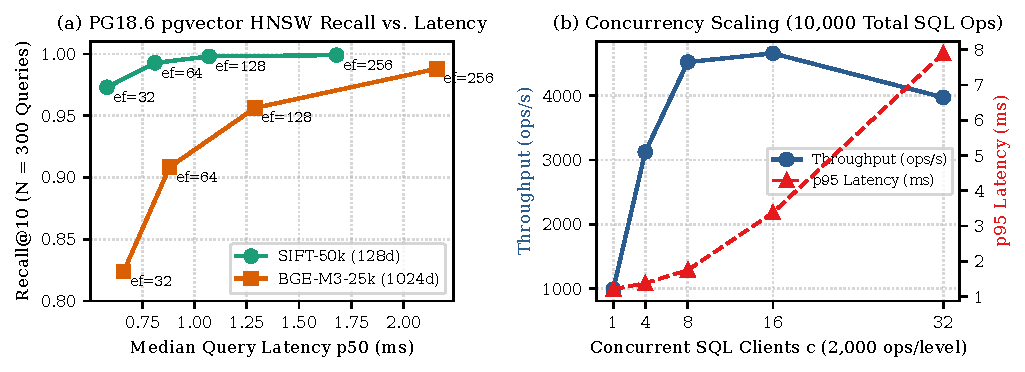
\includegraphics[width=\columnwidth]{figures/fig4_pg18_hnsw_concurrency.pdf}
\caption{PostgreSQL~18.6 HNSW empirical performance: (a)~Recall@10 versus median latency across \texttt{ef\_search} $\in \{32,64,128,256\}$; (b)~throughput and p95 latency across $c \in \{1,4,8,16,32\}$ with 2,000 real SQL queries per level.}
\label{fig:hnsw}
\end{figure}

\section{Coordinate-Confidential CKKS Tier: True 1-CT Aggregation and Scaling Limits}
\subsection{Cryptographic Cost of Server-Side 1-CT Slot Aggregation}
In SIMD-packed \texttt{RNS-CKKS} ($d=128$), a ring of dimension $N$ provides $S = N/2$ complex slots, packing $v = S/128$ vectors per ciphertext ($v=16$ on $N=4096$; $v=32$ on $N=8192$). Evaluating $M = 224$ candidates requires $G = \lceil M/v \rceil$ blocks ($G=14$ on $N=4096$; $G=7$ on $N=8192$). In \texttt{Multi-CT} mode, the server multiplies $\mathrm{EvalMult}(\mathrm{ct}_q, \mathrm{pt}_{D_g})$, performs $\log_2(128) = 7$ rotations and additions, compresses to level~1, and returns all $G$ ciphertexts. This consumes multiplicative depth $L=1$, fitting within $N=4096$ (\texttt{BV} key-switching, $\log_2 Q = 84 \le 109$~bits under \texttt{HEStd\_128\_classic}), but transmits **909.3~KB** per response and forces the client to execute $G=14$ separate decryptions.

To return a \emph{single} ciphertext (\texttt{True 1-CT}), one cannot simply rotate and sum $\mathrm{ct}_{\text{ip}}^{(g)}$ directly because intra-block sliding-window sums leave non-zero cross-vector residuals in slots $128j + u$ ($u \ge 1$). Exact 1-CT aggregation requires multiplying each block by a binary indicator mask $\mathbf{m}_0$ ($m_0[128j] = 1$, $0$ elsewhere), rotating by $-g$ via power-of-two rotation keys, and summing $\mathrm{ct}_{\text{agg}} = \sum_{g=0}^{G-1} \mathrm{EvalRotate}(\mathrm{EvalMult}(\mathrm{ct}_{\text{ip}}^{(g)}, \mathbf{m}_0), -g)$. This consumes multiplicative depth $L=2$. Under \texttt{HEStd\_128\_classic}, $N=4096$ caps $\log_2(QP) \le 109$~bits, leaving insufficient precision per prime for two rescales without RNS approximation overflow. Promoting 1-CT to **$N=8192$** (\texttt{FIXEDAUTO}, primes $(56,42,42)$~bits, $\log_2 Q = 140 \le 218$~bits, $G=7$ blocks) preserves inner-product precision ($\max|\Delta\text{IP}| \le 1.6 \times 10^{-3}$) while compressing response wire size $7.05\times$ to **129.0~KB** and reducing client decryption $5.56\times$ (3.28 to 0.59~ms), while explicitly increasing server compute from 11.23~ms to 27.33~ms (21.60~ms IP + 5.57~ms mask/rotate/sum).

\begin{figure}[!t]
\centering
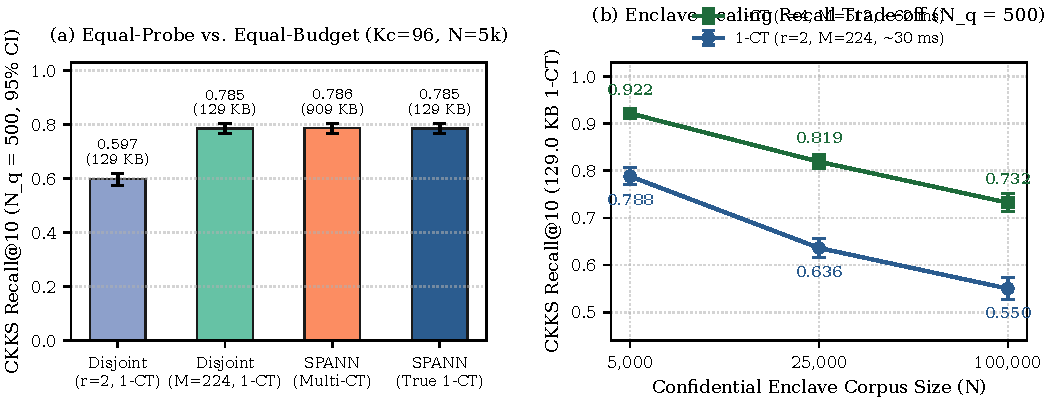
\includegraphics[width=\columnwidth]{figures/fig3_ckks_1ct_and_scaling.pdf}
\caption{Real C++ \texttt{OpenFHE} evaluation across $N_q = 500$ SIFT-1M queries: (a)~controlled $K_c=96$ comparison across equal-probe, equal-budget, \texttt{Multi-CT}, and \texttt{True 1-CT}; (b)~enclave scaling from 5,000 to 100,000 vectors showing full Recall@10 confidence intervals for $M=224$ ($r=2$) and $M=512$ ($r=4$) inside a single 129.0~KB return ciphertext.}
\label{fig:ckks}
\end{figure}

\begin{table*}[!t]
\centering
\caption{Controlled Confidential CKKS Audit on Genuine SIFT-1M ($N=5,000, N_q=500$ Queries): Equal-Probe vs.\ Equal-Candidate-Budget and \texttt{Multi-CT} vs.\ \texttt{True 1-CT}}
\label{tab:ckks_ctrl}
\footnotesize
\begin{adjustbox}{max width=\textwidth}
\begin{tabular}{clrcrrrrrr}
\toprule
$\boldsymbol{K_c}$ & \textbf{Partitioning \& Return Scheme} & \textbf{Ring $N$} & \textbf{Slots (Uniq.)} & \textbf{Recall@10 [95\% CI]} & \textbf{Enc (ms)} & \textbf{Srv IP + Agg (ms)} & \textbf{Dec (ms)} & \textbf{Total (ms)} & \textbf{Resp (KB)} \\
\midrule
96 & Disjoint Equal-Probe ($r=2$, 1-CT) & 8192 & 113.3 (113.3) & 0.5968 [0.5744, 0.6192] & 2.59 & 12.31 + 3.51 & 0.54 & 19.30 & 129.0 \\
96 & Disjoint Equal-Budget ($M=224$, 1-CT) & 8192 & 224.0 (224.0) & 0.7846 [0.7672, 0.8020] & 2.64 & 21.05 + 5.41 & 0.57 & 29.84 & 129.0 \\
96 & SPANN Padded ($r=2$, Multi-CT) & 4096 & 224.0 (202.3) & 0.7856 [0.7673, 0.8039] & 1.02 & 8.86 + 2.36 & 3.28 & 15.55 & 909.3 \\
96 & SPANN Padded ($r=2$, Multi-CT) & 8192 & 224.0 (202.3) & 0.7838 [0.7656, 0.8020] & 1.98 & 9.34 + 2.57 & 3.48 & 17.47 & 902.7 \\
96 & SPANN Padded ($r=2$, True 1-CT) & 8192 & 224.0 (202.3) & 0.7852 [0.7670, 0.8034] & 2.72 & 21.60 + 5.57 & 0.59 & 30.66 & 129.0 \\
\midrule
192 & Disjoint Equal-Probe ($r=2$, 1-CT) & 8192 & 64.7 (64.7) & 0.5332 [0.5110, 0.5554] & 2.51 & 9.90 + 2.37 & 0.52 & 15.44 & 129.0 \\
192 & Disjoint Equal-Budget ($M=224$, 1-CT) & 8192 & 224.0 (224.0) & 0.8498 [0.8354, 0.8642] & 2.73 & 21.47 + 5.54 & 0.58 & 30.55 & 129.0 \\
192 & SPANN Padded ($r=2$, Multi-CT) & 4096 & 224.0 (155.5) & 0.7618 [0.7425, 0.7811] & 1.02 & 8.93 + 2.36 & 3.31 & 15.70 & 909.3 \\
192 & SPANN Padded ($r=2$, Multi-CT) & 8192 & 224.0 (155.5) & 0.7608 [0.7416, 0.7800] & 2.01 & 9.36 + 2.57 & 3.50 & 17.50 & 902.7 \\
192 & SPANN Padded ($r=2$, True 1-CT) & 8192 & 224.0 (155.5) & 0.7612 [0.7420, 0.7804] & 2.72 & 21.59 + 5.58 & 0.58 & 30.60 & 129.0 \\
\bottomrule
\end{tabular}
\end{adjustbox}
\end{table*}

\begin{table*}[!t]
\centering
\caption{Confidential Enclave Scaling ($5,000 \to 25,000 \to 100,000$ Genuine SIFT-1M Vectors, $N_q=500$ Queries) Reporting Full Recall@10 Confidence Intervals}
\label{tab:ckks_scale}
\footnotesize
\begin{adjustbox}{max width=\textwidth}
\begin{tabular}{rrlcrrrr}
\toprule
\textbf{Enclave $N$} & $\boldsymbol{K_c}$ & \textbf{CKKS Evaluation Profile} & \textbf{Recall@10 [95\% CI]} & \textbf{Srv IP + Agg (ms)} & \textbf{Dec (ms)} & \textbf{Total E2E (ms)} & \textbf{Resp (KB)} \\
\midrule
5,000 & 96 & Multi-CT ($r=2, M=224, N=4096$) & \textbf{0.7890} [0.7712, 0.8068] & 9.09 + 2.38 & 3.40 & 15.99 & 909.3 \\
5,000 & 96 & True 1-CT ($r=2, M=224, N=8192$) & \textbf{0.7882} [0.7704, 0.8060] & 21.69 + 5.64 & 0.58 & 30.99 & 129.0 \\
5,000 & 96 & True 1-CT ($r=4, M=512, N=8192$) & \textbf{0.9216} [0.9112, 0.9320] & 45.23 + 14.95 & 0.60 & 63.79 & 129.0 \\
\midrule
25,000 & 384 & Multi-CT ($r=2, M=224, N=4096$) & \textbf{0.6368} [0.6160, 0.6576] & 9.20 + 2.35 & 3.29 & 15.98 & 909.3 \\
25,000 & 384 & True 1-CT ($r=2, M=224, N=8192$) & \textbf{0.6364} [0.6156, 0.6572] & 20.95 + 5.48 & 0.57 & 30.09 & 129.0 \\
25,000 & 384 & True 1-CT ($r=4, M=512, N=8192$) & \textbf{0.8192} [0.8043, 0.8341] & 45.00 + 14.95 & 0.60 & 63.54 & 129.0 \\
\midrule
100,000 & 1280 & Multi-CT ($r=2, M=224, N=4096$) & \textbf{0.5504} [0.5277, 0.5731] & 9.25 + 2.33 & 3.25 & 16.08 & 909.3 \\
100,000 & 1280 & True 1-CT ($r=2, M=224, N=8192$) & \textbf{0.5502} [0.5275, 0.5729] & 20.81 + 5.41 & 0.57 & 29.85 & 129.0 \\
100,000 & 1280 & True 1-CT ($r=4, M=512, N=8192$) & \textbf{0.7322} [0.7132, 0.7512] & 43.50 + 14.32 & 0.59 & 61.44 & 129.0 \\
\bottomrule
\end{tabular}
\end{adjustbox}
\end{table*}

\subsection{Equal-Probe vs.\ Equal-Budget and 100k Recall Scaling}
Tables~\ref{tab:ckks_ctrl}--\ref{tab:ckks_scale} and Fig.~\ref{fig:ckks} resolve two essential methodological questions over $N_q = 500$ real queries:
\begin{enumerate}
\item \textbf{Equal-Probe vs.\ Equal-Budget:} At $K_c=96$, constant-padded \texttt{SPANN} ($r=2, B_{\max}=112$) improves Recall@10 over equal-probe disjoint K-means by $+0.1884$ (0.7852 vs.\ 0.5968, Wilcoxon $p = 2.58 \times 10^{-65}$). However, when disjoint K-means is granted an identical 224-vector candidate budget by probing variable numbers of clusters per query, it achieves 0.7846 ($p = 0.75$ at $K_c=96$; $0.8498$ vs.\ $0.7612$ at $K_c=192$) because constant-padded \texttt{SPANN} dedicates slots to boundary replicas and zero-padding. Variable-probe disjoint routing, however, leaks query-dependent cluster counts $r(q)$ and exact bucket sizes $|B_k|$ to the cloud server, whereas padded \texttt{SPANN} enforces constant work ($M=224$) and zero bucket-size leakage.
\item \textbf{Candid Recall Scaling to 100,000 Vectors:} Maintaining fixed $M=224$ ($r=2$) yields $O(1)$ server evaluation latency (27.58--26.45~ms, total E2E 29.85~ms at $N=100,000$), but Recall@10 drops from **0.7882** ($N=5\text{k}$) to **0.6364** ($N=25\text{k}$) and **0.5502** ($N=100\text{k}$), falling below the $0.92$ public-tier target. Expanding to $r=4, B_{\max}=128$ ($M=512$ candidates packed into the \emph{same} 129.0~KB 1-CT response) recovers Recall@10 to **0.9216** ($5\text{k}$), **0.8192** ($25\text{k}$), and **0.7322** ($100\text{k}$) at 61.44~ms E2E latency. Sustaining $\ge 0.90$ recall at $10^5+$ scale requires multi-ciphertext candidate budgets ($M \ge 1,536$) or hierarchical encrypted re-ranking.
\end{enumerate}

\section{Lagged 5D Contextual Control and Silicon Energy Metrology}
\subsection{Mean-Centered Russac D-LinUCB with Full 5D Context}
Prior to executing query $q_t$, the edge controller observes a strictly non-anticipative lagged five-dimensional context vector:
\begin{equation}
\mathbf{x}_{t^-} = \left[\,1,\; \mathbb{I}_{\text{sql}}(q_t),\; \mathbb{I}_{\text{conf}}(q_t),\; \min\!\left(\frac{\widehat{\text{RTT}}_{t^-}}{300}, 2\right),\; \min\!\left(\frac{\widehat{\text{loss}}_{t^-}}{0.10}, 2\right)\right]^\top \in \mathbb{R}^5.
\end{equation}
Notably, \emph{no observable network features are withheld from stationary or sliding-window baselines}. All controllers share a frozen configuration (\nolinkurl{v5_bandit_frozen_config.json}: discount $\gamma = 0.88$, exploration $\nu = 0.06$, ridge $\lambda = 0.08$, neutral prior $\mu_0 = 0.48$, window $W = 32$, loss weights $w_L = 0.45, w_A = 0.55, w_V = 0.85$). For arm $a$, Russac's discounted covariance~\cite{russac2019dlinucb} updates via $\mathbf{V}_{t,a} = \gamma \mathbf{V}_{t-1,a} + \mathbf{x}_{t^-}\mathbf{x}_{t^-}^\top + (1-\gamma)\lambda \mathbf{I}_5$, $\tilde{\mathbf{V}}_{t,a} = \gamma^2 \tilde{\mathbf{V}}_{t-1,a} + \mathbf{x}_{t^-}\mathbf{x}_{t^-}^\top + (1-\gamma^2)\lambda \mathbf{I}_5$, and mean-centered target $\mathbf{b}_{t,a} = \gamma \mathbf{b}_{t-1,a} + (\ell_{t,a} - \mu_0)\mathbf{x}_{t^-}$, selecting among accuracy-feasible arms the minimum lower confidence bound $\hat{\theta}_{t,a}^\top \mathbf{x}_{t^-} - \nu \sqrt{\mathbf{x}_{t^-}^\top \mathbf{V}_{t,a}^{-1} \tilde{\mathbf{V}}_{t,a} \mathbf{V}_{t,a}^{-1} \mathbf{x}_{t^-}}$.

\begin{figure}[!t]
\centering
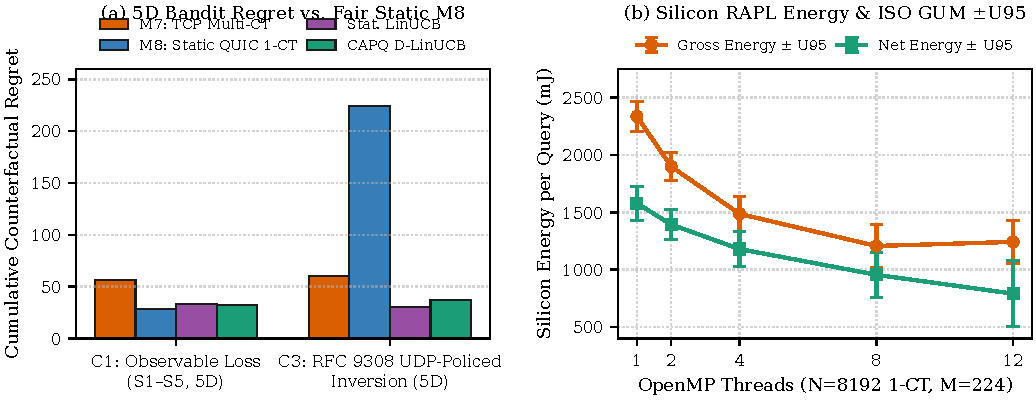
\includegraphics[width=\columnwidth]{figures/fig5_bandit_and_rapl_energy.pdf}
\caption{(a)~5D contextual bandit cumulative regret against fair static \texttt{M8} across observable loss shifts and RFC~9308 UDP-policed inversions (10 seeds); (b)~silicon RAPL (\nolinkurl{rapl_package0_pkg}) gross and net query energy with ISO GUM $\pm U_{95}$ uncertainty across OpenMP threads.}
\label{fig:bandit_rapl}
\end{figure}

\begin{table*}[!t]
\centering
\caption{Silicon RAPL (\texttt{rapl\_package0\_pkg}) Steady-State OpenMP Scaling and ISO GUM $\pm U_{95}$ Uncertainty ($N=8192$ True 1-CT Enclave)}
\label{tab:rapl}
\footnotesize
\begin{adjustbox}{max width=\textwidth}
\begin{tabular}{lrrrrrrrr}
\toprule
\textbf{Enclave Workload} & \textbf{OMP Threads} & \textbf{Steady Ops} & \textbf{Med Lat (ms)} & \textbf{Throughput (q/s)} & \textbf{Active Power (W)} & \textbf{Idle Drift} & \textbf{Gross Energy $\pm U_{95}$ (mJ)} & \textbf{Net Energy $\pm U_{95}$ (mJ)} \\
\midrule
Standard ($M=224, r=2$) & 1 & 57 & 106.63 & 9.41 & 21.99 & -7.3\% & 2336.1 $\pm$ 133.2 & 1580.0 $\pm$ 149.1 \\
Standard ($M=224, r=2$) & 2 & 94 & 65.60 & 15.59 & 29.61 & -2.7\% & 1899.7 $\pm$ 125.5 & 1394.0 $\pm$ 133.8 \\
Standard ($M=224, r=2$) & 4 & 133 & 43.85 & 22.15 & 32.94 & -1.4\% & 1486.9 $\pm$ 153.4 & 1180.7 $\pm$ 155.4 \\
Standard ($M=224, r=2$) & 8 & 148 & 34.82 & 24.50 & 29.57 & -18.6\% & 1207.2 $\pm$ 190.3 & 956.1 $\pm$ 195.4 \\
Standard ($M=224, r=2$) & 12 & 126 & 41.11 & 20.79 & 25.85 & +116.4\% & 1243.1 $\pm$ 184.0 & 791.4 $\pm$ 289.1 \\
\midrule
Heavy ($M=512, r=4$) & 1 & 24 & 253.34 & 3.84 & 20.54 & -66.4\% & 5344.4 $\pm$ 545.2 & 1759.6 $\pm$ 2366.8 \\
Heavy ($M=512, r=4$) & 2 & 41 & 149.00 & 6.69 & 31.50 & -76.9\% & 4709.2 $\pm$ 388.7 & 1562.7 $\pm$ 2493.5 \\
Heavy ($M=512, r=4$) & 4 & 67 & 88.88 & 11.08 & 38.38 & -0.1\% & 3464.2 $\pm$ 210.8 & 2851.0 $\pm$ 239.7 \\
Heavy ($M=512, r=4$) & 8 & 88 & 68.02 & 14.59 & 41.29 & +48.1\% & 2829.2 $\pm$ 124.4 & 2335.5 $\pm$ 215.1 \\
Heavy ($M=512, r=4$) & 12 & 88 & 68.49 & 14.62 & 43.43 & +101.5\% & 2969.7 $\pm$ 171.5 & 2433.1 $\pm$ 330.4 \\
\bottomrule
\end{tabular}
\end{adjustbox}
\end{table*}

\begin{table*}[!t]
\centering
\caption{5D Contextual Bandit Evaluation (10 Seeds, $T=320$/Seed, Frozen $\gamma=0.88, \nu=0.06, \lambda=0.08$) Against Legacy \texttt{M7} and Fair Static \texttt{M8}}
\label{tab:bandit}
\footnotesize
\begin{adjustbox}{max width=\textwidth}
\begin{tabular}{llcrrrr}
\toprule
\textbf{Regime Campaign (Full 5D Context)} & \textbf{Controller / Baseline} & \textbf{Cum.\ Regret [95\% CI]} & \textbf{Mean Lat (ms)} & \textbf{Mean Acc} & \textbf{Class-SLA} & \textbf{Wilcoxon $p$} \\
\midrule
C1: Observable Loss (S1--S5) & M7: Static TCP + Multi-CT & 56.33 [52.50, 60.17] & 1334.73 & 0.9453 & 84.03\% & 0.0059 \\
C1: Observable Loss (S1--S5) & Static TCP + 1-CT & 57.07 [53.05, 61.10] & 537.45 & 0.9453 & 84.03\% & 0.0059 \\
C1: Observable Loss (S1--S5) & M8: Fair Static QUIC + INT8 + 1-CT & 28.60 [26.64, 30.57] & 121.62 & 0.9448 & 89.44\% & 0.2622 \\
C1: Observable Loss (S1--S5) & Stationary LinUCB ($\gamma=1.0$) & 33.39 [27.98, 38.80] & 465.23 & 0.9436 & 87.94\% & 0.5408 \\
C1: Observable Loss (S1--S5) & Sliding-Window LinUCB ($W=32$) & 25.08 [19.56, 30.60] & 237.87 & 0.9422 & 88.22\% & 0.0665 \\
C1: Observable Loss (S1--S5) & CAPQ D-LinUCB ($\gamma=0.88$) & 32.13 [24.52, 39.74] & 301.14 & 0.9424 & 87.09\% & --- \\
\midrule
C2: Backend TCP Queue Stall & M7: Static TCP + Multi-CT & 33.58 [33.50, 33.67] & 57.67 & 0.9453 & 100.00\% & 0.0323 \\
C2: Backend TCP Queue Stall & Static TCP + 1-CT & 36.08 [35.51, 36.66] & 61.57 & 0.9453 & 99.91\% & 0.0059 \\
C2: Backend TCP Queue Stall & M8: Fair Static QUIC + INT8 + 1-CT & 6.75 [6.74, 6.77] & 27.00 & 0.9448 & 100.00\% & 0.0059 \\
C2: Backend TCP Queue Stall & Stationary LinUCB ($\gamma=1.0$) & 29.63 [27.36, 31.89] & 44.59 & 0.9422 & 98.69\% & 0.9188 \\
C2: Backend TCP Queue Stall & Sliding-Window LinUCB ($W=32$) & 29.48 [27.57, 31.40] & 41.90 & 0.9409 & 98.12\% & 1.0000 \\
C2: Backend TCP Queue Stall & CAPQ D-LinUCB ($\gamma=0.88$) & 30.09 [27.39, 32.78] & 45.41 & 0.9421 & 98.62\% & --- \\
\midrule
C3: RFC 9308 UDP Policing & M7: Static TCP + Multi-CT & 60.56 [57.51, 63.60] & 182.99 & 0.9453 & 87.66\% & 0.0415 \\
C3: RFC 9308 UDP Policing & Static TCP + 1-CT & 70.47 [67.12, 73.82] & 119.83 & 0.9453 & 86.72\% & 0.0080 \\
C3: RFC 9308 UDP Policing & M8: Fair Static QUIC + INT8 + 1-CT & 224.48 [222.97, 225.99] & 999.21 & 0.9448 & 57.81\% & 0.0059 \\
C3: RFC 9308 UDP Policing & Stationary LinUCB ($\gamma=1.0$) & 30.09 [18.06, 42.11] & 141.59 & 0.9446 & 94.47\% & 0.0191 \\
C3: RFC 9308 UDP Policing & Sliding-Window LinUCB ($W=32$) & 34.25 [18.81, 49.70] & 155.43 & 0.9437 & 93.03\% & 0.1851 \\
C3: RFC 9308 UDP Policing & CAPQ D-LinUCB ($\gamma=0.88$) & 37.21 [22.82, 51.60] & 159.29 & 0.9437 & 92.69\% & --- \\
\bottomrule
\end{tabular}
\end{adjustbox}
\end{table*}

\subsection{Candid Bandit Findings and Silicon RAPL Metrology}
Table~\ref{tab:bandit} and Fig.~\ref{fig:bandit_rapl}(a) establish a clear operational boundary:
\begin{itemize}
\item \textbf{Unimpaired / Observable Lossy Paths (C1 \& C2):} Once \texttt{M8} is equipped with warm QUIC, \texttt{INT8}, \texttt{SPANN}, and 1-CT aggregation, \texttt{M8} achieves the lowest latency (121.62~ms in C1; 27.00~ms in C2) and highest SLA (89.44\% and 100.00\%). Because online bandits incur initial exploration across slower TCP arms, \texttt{CAPQ D-LinUCB} exhibits statistically indistinguishable regret from \texttt{M8} in C1 (32.13 vs.\ 28.60, $p = 0.2622$) but higher mean latency (301.14~ms), and matches stationary/SW-LinUCB ($p \ge 0.066$).
\item \textbf{RFC 9308 Enterprise UDP Policing Inversion (C3):} When paths alternate between wireless packet loss (where QUIC excels) and enterprise middleboxes applying token-bucket UDP policing~\cite{rfc9308} (where \texttt{M8} degrades to 999.21~ms and 57.81\% SLA, regret 224.48), contextual bandits automatically fall back to pooled \texttt{TCP+1-CT}, restoring SLA compliance to **92.69\%--94.47\%** and cutting regret by $6\times$ ($p = 0.0059$). Thus, the bandit serves specifically as a transport-safety fallback rather than outperforming static QUIC on open links.
\end{itemize}

Table~\ref{tab:rapl} and Fig.~\ref{fig:bandit_rapl}(b) report steady-state 6-second continuous C++ \texttt{OpenFHE} execution measured directly from Intel Meteor Lake silicon package counters (\nolinkurl{rapl_package0_pkg} via \nolinkurl{PDH_FMT_LARGE}, $\kappa_E = 3.6 \times 10^{-6}$~mJ/pWh) with pre/post quiescent C-state settling ($\le 8.8$~W). Propagating pre-to-post idle drift $\Delta P_{\text{drift}}$ via ISO GUM rectangular Type-B variance $(\Delta P_{\text{drift}})^2/12$~\cite{iso_gum_2008}, $N=8192$ 1-CT scales cleanly from 106.63~ms (\texttt{OMP}=1, gross $2,336.1 \pm 133.2$~mJ, net $1,580.1 \pm 149.1$~mJ) down to **34.82~ms at \texttt{OMP}=8** (24.50~q/s, gross $1,207.2 \pm 190.3$~mJ, net $956.1 \pm 195.4$~mJ) before thread-synchronization overhead and hybrid E-core scheduling increase latency to 41.11~ms and widen idle drift at \texttt{OMP}=12. On ARM64 cloud silicon (\texttt{GCP t2a-standard-4}, Ampere Altra Neoverse-N1), cross-ISA execution confirms portable sub-millisecond PQC handshakes and consistent \texttt{OpenFHE} RNS-CKKS numerical parity.

\section{Factorial Attribution and Dual-Track Multi-Region WAN Evaluation}
\subsection{\texorpdfstring{$2^5$}{2\textasciicircum 5} Factorial GLM and Exact 10,000-Block Permutations}
Table~\ref{tab:glm} and Fig.~\ref{fig:glm} evaluate all 32 configurations of the $2^5$ full-factorial design ($N=256$ blocked runs) using both HC3-robust Binomial Logit GLM and an exact distribution-free 10,000 within-block permutation test. Session pooling (Factor~A, $+52.15$~pp SLA) is overwhelmingly the dominant system driver under both parametric GLM ($p < 0.0001$) and exact block permutation ($p = 0.0001$, Holm-5 $p = 0.0005$). By contrast, while Factors~D ($+8.40$~pp) and~E ($+8.01$~pp) appear highly significant under parametric GLM ($p \le 0.0003$), exact block permutation yields raw $p = 0.0385$ and $p = 0.0518$ (Holm-5 $p = 0.1540$ and $0.1554$), confirming that online control is a secondary contributor relative to session pooling. For Factor~B (\texttt{SPANN} replication), the overall 4-class mixture accuracy gain of $+0.0333$ corresponds directly to $+0.0333 / 0.25 = +0.1334$ on the 25\% confidential query subset.

\begin{figure}[!t]
\centering
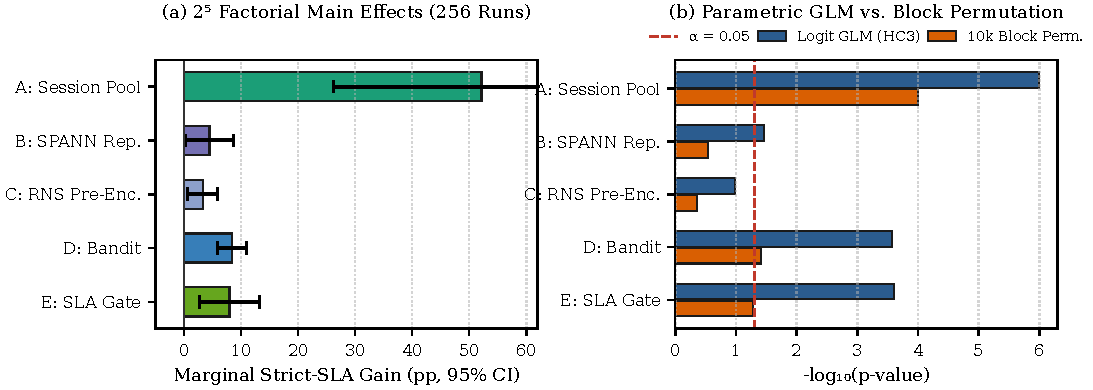
\includegraphics[width=\columnwidth]{figures/fig6_factorial_glm_permutation.pdf}
\caption{$2^5$ full-factorial attribution ($N=256$ runs): (a)~marginal SLA effects with 95\% block CIs; (b)~comparison of HC3 Binomial Logit GLM versus exact 10,000 within-block permutation $-\log_{10}(p)$ values.}
\label{fig:glm}
\end{figure}

\begin{table*}[!t]
\centering
\caption{$2^5$ Full-Factorial Attribution ($N=256$ Cells): HC3 Binomial Logit GLM vs.\ Exact 10,000 Within-Block Permutation Verification}
\label{tab:glm}
\footnotesize
\begin{adjustbox}{max width=\textwidth}
\begin{tabular}{lcccccc}
\toprule
\textbf{Architectural Factor} & \textbf{$\Delta$SLA (pp) [95\% CI]} & \textbf{Logit $\hat{\beta}$ (HC3 SE)} & \textbf{GLM $p$} & \textbf{Perm-10k $p$} & \textbf{Perm Holm-5} & \textbf{$\Delta$Acc Mix (Conf.\ Tier)} \\
\midrule
A PQC Session Pooling & +52.15 [+26.18, +78.11] & +2.974 (0.199) & $<0.0001$ & 0.0001 & 0.0005 & +0.0000 (N/A) \\
B SPANN Boundary Replication & +4.49 [+0.34, +8.65] & +0.281 (0.133) & 0.0348 & 0.2851 & 0.57014 & +0.0333 (0.1334) \\
C SIMD RNS PreEncoding & +3.32 [+0.67, +5.97] & +0.218 (0.134) & 0.1025 & 0.4363 & 0.57014 & -0.0000 (N/A) \\
D Lagged Discounted Bandit & +8.40 [+5.89, +10.91] & +0.485 (0.133) & 0.0003 & 0.0385 & 0.15398 & -0.0133 (N/A) \\
E Dual SLA Feasibility Gate & +8.01 [+2.81, +13.21] & +0.486 (0.133) & 0.0002 & 0.0518 & 0.15538 & +0.0573 (N/A) \\
\bottomrule
\end{tabular}
\end{adjustbox}
\end{table*}

\subsection{Dual-Track 3-Region WAN Evaluation and 4D Pareto Analysis}
To guarantee strict single-campaign statistical pairing without mixing runs across time, Tables~\ref{tab:wan_live}--\ref{tab:wan_ctrl} and Figs.~\ref{fig:wan}--\ref{fig:pareto} report two provenance-locked multi-region tracks:

\begin{enumerate}
\item \textbf{Track 1 --- Pure Live 3-Region GCP Campaign (\texttt{M1--M5}, 1,440 Interleaved Queries, Table~\ref{tab:wan_live}):} Executed simultaneously via Latin-square interleaving from Thailand to \texttt{n4-standard-4} instances in Bangkok (9.8~ms 1-RTT), Singapore (56.1~ms), and US-Central (225.5~ms). Compared to fresh per-query PQC (\texttt{M1}), \texttt{M5} cuts mean latency by **61.9\%** in Bangkok (126.89 to 48.35~ms), **70.9\%** in Singapore (266.33 to 77.63~ms), and **72.8\%** in US-Central (971.24 to 264.42~ms), while reducing edge energy in Singapore from 1,339.1 to 580.7~mJ. On the 24 confidential queries per region, live 250~ms SLA rises from 62.5\% to 91.7\% in Bangkok and from 4.2\% to 91.7\% in Singapore, whereas in US-Central (225.5~ms 1-RTT) all modes achieve 0.0\% 250~ms SLA due to physical propagation delay.
\item \textbf{Track 2 --- Controlled 3-Region Calibrated \texttt{netns} Campaign (\texttt{M1--M8}, 2,304 Interleaved Queries, Table~\ref{tab:wan_ctrl}):} Evaluates all eight modes in a single interleaved campaign calibrated to the three regional RTTs with 0.15\%--0.30\% packet loss and full $N=8192$ 1-CT / $N=4096$ Multi-CT wire payloads. In Singapore (56.1~ms, 0.25\% loss), legacy \texttt{M7} (\texttt{TCP + Multi-CT}, 909.3~KB) suffers TCP head-of-line blocking, averaging **359.61~ms** (p95 $= 1,736.36$~ms, confidential 250~ms SLA $= 8.3\%$, egress+compute cost $\$27.47$/1M). Both fair static \texttt{M8} (**92.04~ms**, confidential SLA $= 79.2\%$, $\$13.86$/1M) and adaptive \texttt{M5} (**94.67~ms**, confidential SLA $= 79.2\%$, $\$13.89$/1M) cut latency by $3.8\times$ and halve cloud egress cost. Across the 4D objective vector (Latency, Edge Energy, Cloud Cost, $1-\text{Accuracy}$), \texttt{M4}, \texttt{M6}, \texttt{M7}, \texttt{M8}, and \texttt{M5} all reside on the non-dominated Pareto frontier: \texttt{M7} retains slightly higher raw precision ($0.9454$ vs.\ $0.9448$/$0.9453$) at $2\times$ monetary cost and $3.8\times$ latency, while \texttt{M8} and \texttt{M5} co-occupy the low-latency, low-egress knee.
\end{enumerate}

\begin{figure}[!t]
\centering
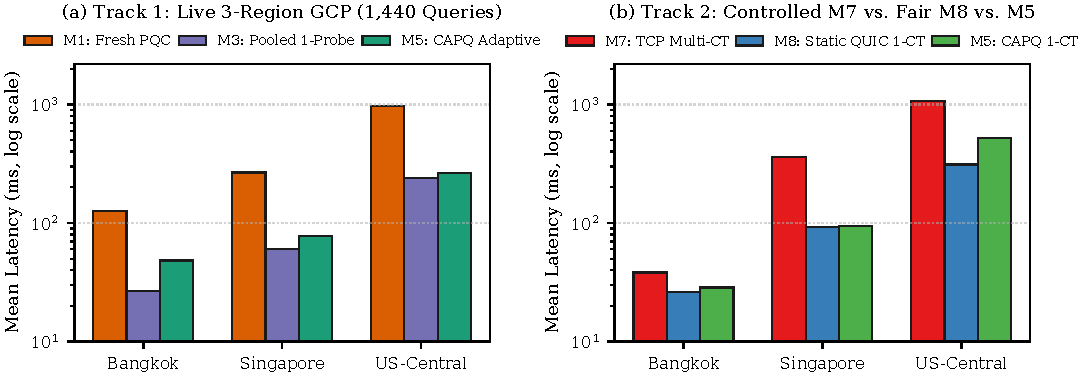
\includegraphics[width=\columnwidth]{figures/fig7_dual_track_wan_latency.pdf}
\caption{Multi-region WAN mean latency (log scale): (a)~Track~1 pure live GCP campaign (\texttt{M1--M5}, 1,440 queries); (b)~Track~2 controlled 3-region campaign comparing \texttt{M7} (\texttt{Multi-CT}) against fair static \texttt{M8} and adaptive \texttt{M5} (2,304 queries).}
\label{fig:wan}
\end{figure}

\begin{figure}[!t]
\centering
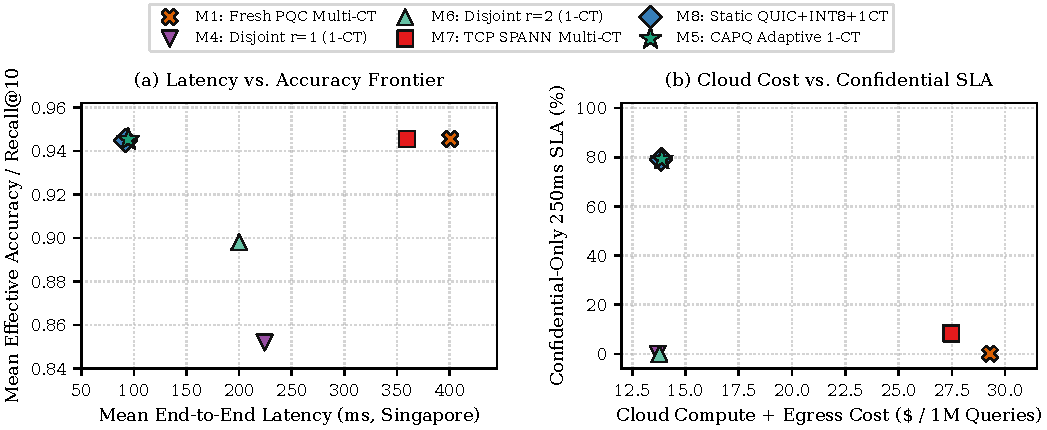
\includegraphics[width=\columnwidth]{figures/fig8_pareto_4d_cost_conf_sla.pdf}
\caption{4D Pareto trade-offs in the Singapore regional profile (56.1~ms 1-RTT, 0.25\% loss): (a)~mean latency versus effective accuracy; (b)~cloud compute+egress cost versus confidential-only 250~ms SLA pass rate.}
\label{fig:pareto}
\end{figure}

\begin{table*}[!t]
\centering
\caption{Track 1: Pure Live 3-Region GCP Interleaved Campaign (\texttt{M1--M5}, 1,440 Raw Queries on \texttt{n4-standard-4}) Reporting MBB 95\% CIs, Energy, Cost, and Confidential-Only SLA}
\label{tab:wan_live}
\footnotesize
\begin{adjustbox}{max width=\textwidth}
\begin{tabular}{llcrrrrrr}
\toprule
\textbf{Region (1-RTT)} & \textbf{System Mode} & \textbf{Mean Lat [MBB 95\% CI] (ms)} & \textbf{p95 (ms)} & \textbf{Mean Acc} & \textbf{Energy (mJ)} & \textbf{Cost / 1M} & \textbf{Strict-150} & \textbf{Class-250 (Conf-Only)} \\
\midrule
Bangkok (9.8~ms) & M1: Fresh Hybrid-PQC TLS 1.3 & 126.89 [111.8, 145.0] & 296.0 & 0.9844 & 513.6 & \$1.112 & 61.5\% & 76.0\% (62.5\%) \\
Bangkok (9.8~ms) & M2: Pooled Classical TLS (Non-Conf.) & 23.81 [18.6, 28.7] & 72.1 & 0.7438 & 65.8 & \$0.093 & 68.8\% & 68.8\% (0.0\%) \\
Bangkok (9.8~ms) & M3: Pooled PQC Single-Probe & 26.92 [23.5, 30.4] & 74.3 & 0.8656 & 107.7 & \$0.246 & 70.8\% & 74.0\% (20.8\%) \\
Bangkok (9.8~ms) & M4: Pooled PQC Static Heuristic & 25.86 [21.6, 32.3] & 71.9 & 0.8646 & 100.7 & \$0.248 & 68.8\% & 71.9\% (20.8\%) \\
Bangkok (9.8~ms) & M5: CAPQ-Pareto Adaptive & 48.35 [43.3, 54.7] & 170.0 & 0.9802 & 388.4 & \$0.969 & 78.1\% & 90.6\% (91.7\%) \\
\midrule
Singapore (56.0~ms) & M1: Fresh Hybrid-PQC TLS 1.3 & 266.33 [228.2, 284.7] & 414.3 & 0.9865 & 1339.1 & \$1.070 & 2.1\% & 3.1\% (4.2\%) \\
Singapore (56.0~ms) & M2: Pooled Classical TLS (Non-Conf.) & 49.37 [44.0, 52.9] & 93.7 & 0.7458 & 145.5 & \$0.089 & 70.8\% & 70.8\% (0.0\%) \\
Singapore (56.0~ms) & M3: Pooled PQC Single-Probe & 60.23 [55.2, 66.2] & 121.3 & 0.8677 & 242.7 & \$0.237 & 72.9\% & 76.0\% (20.8\%) \\
Singapore (56.0~ms) & M4: Pooled PQC Static Heuristic & 62.43 [54.3, 71.8] & 125.3 & 0.8656 & 272.4 & \$0.242 & 68.8\% & 71.9\% (20.8\%) \\
Singapore (56.0~ms) & M5: CAPQ-Pareto Adaptive & 77.63 [71.2, 84.2] & 202.6 & 0.9813 & 580.7 & \$0.938 & 75.0\% & 91.7\% (91.7\%) \\
\midrule
US-Central (225.5~ms) & M1: Fresh Hybrid-PQC TLS 1.3 & 971.24 [962.2, 986.5] & 1100.9 & 0.9865 & 84.7 & \$1.015 & 0.0\% & 0.0\% (0.0\%) \\
US-Central (225.5~ms) & M2: Pooled Classical TLS (Non-Conf.) & 229.15 [228.3, 229.9] & 237.4 & 0.7458 & 19.1 & \$0.084 & 0.0\% & 0.0\% (0.0\%) \\
US-Central (225.5~ms) & M3: Pooled PQC Single-Probe & 239.15 [236.8, 242.7] & 266.6 & 0.8677 & 32.0 & \$0.220 & 0.0\% & 0.0\% (0.0\%) \\
US-Central (225.5~ms) & M4: Pooled PQC Static Heuristic & 240.65 [236.5, 247.8] & 262.2 & 0.8667 & 14.6 & \$0.222 & 0.0\% & 0.0\% (0.0\%) \\
US-Central (225.5~ms) & M5: CAPQ-Pareto Adaptive & 264.42 [256.0, 277.6] & 387.9 & 0.9823 & 46.4 & \$0.885 & 0.0\% & 0.0\% (0.0\%) \\
\bottomrule
\end{tabular}
\end{adjustbox}
\end{table*}

\begin{table*}[!t]
\centering
\caption{Track 2: Controlled 3-Region Calibrated \texttt{netns} Interleaved Campaign (Confidential Modes, 2,304 Queries) Comparing \texttt{M7} (\texttt{Multi-CT}) vs.\ Fair Static \texttt{M8} and Adaptive \texttt{M5}}
\label{tab:wan_ctrl}
\footnotesize
\begin{adjustbox}{max width=\textwidth}
\begin{tabular}{llrrrrrrc}
\toprule
\textbf{Region Profile} & \textbf{Confidential Mode} & \textbf{Mean Lat (ms)} & \textbf{p95 (ms)} & \textbf{Mean Acc} & \textbf{Energy (mJ)} & \textbf{Cost / 1M} & \textbf{Class-250 (Conf-Only)} & \textbf{4D Pareto} \\
\midrule
Bangkok & M1: Fresh PQC + Multi-CT & 69.83 & 146.25 & 0.9454 & 88.2 & \$29.33 & 98.96\% (100.0\%) & No \\
Bangkok & M4: Pooled TCP Disjoint $r=1$ (1-CT) & 22.21 & 57.07 & 0.8520 & 34.7 & \$13.73 & 75.00\% (0.0\%) & Yes \\
Bangkok & M6: Pooled TCP Disjoint $r=2$ (1-CT) & 25.13 & 63.57 & 0.8982 & 45.4 & \$13.83 & 73.96\% (0.0\%) & Yes \\
Bangkok & M7: Pooled TCP SPANN Multi-CT & 38.33 & 136.66 & 0.9454 & 73.4 & \$27.52 & 100.00\% (100.0\%) & Yes \\
Bangkok & M8: Fair Static QUIC+INT8+SPANN+1-CT & 26.37 & 81.54 & 0.9448 & 45.3 & \$13.96 & 100.00\% (100.0\%) & Yes \\
Bangkok & M5: CAPQ-Pareto Adaptive 1-CT & 28.57 & 77.50 & 0.9453 & 45.4 & \$13.99 & 98.96\% (100.0\%) & Yes \\
\midrule
Singapore & M1: Fresh PQC + Multi-CT & 400.90 & 905.75 & 0.9454 & 88.2 & \$29.29 & 0.00\% (0.0\%) & No \\
Singapore & M4: Pooled TCP Disjoint $r=1$ (1-CT) & 224.26 & 808.11 & 0.8520 & 34.7 & \$13.70 & 75.00\% (0.0\%) & Yes \\
Singapore & M6: Pooled TCP Disjoint $r=2$ (1-CT) & 200.15 & 840.92 & 0.8982 & 45.4 & \$13.77 & 73.96\% (0.0\%) & Yes \\
Singapore & M7: Pooled TCP SPANN Multi-CT & 359.61 & 1736.36 & 0.9454 & 73.4 & \$27.47 & 77.08\% (8.3\%) & Yes \\
Singapore & M8: Fair Static QUIC+INT8+SPANN+1-CT & 92.04 & 212.77 & 0.9448 & 45.3 & \$13.86 & 94.79\% (79.2\%) & Yes \\
Singapore & M5: CAPQ-Pareto Adaptive 1-CT & 94.67 & 211.88 & 0.9453 & 45.4 & \$13.89 & 94.79\% (79.2\%) & Yes \\
\midrule
US-Central & M1: Fresh PQC + Multi-CT & 1472.44 & 3046.06 & 0.9454 & 88.2 & \$22.65 & 0.00\% (0.0\%) & No \\
US-Central & M4: Pooled TCP Disjoint $r=1$ (1-CT) & 856.40 & 3436.08 & 0.8520 & 34.7 & \$10.60 & 0.00\% (0.0\%) & Yes \\
US-Central & M6: Pooled TCP Disjoint $r=2$ (1-CT) & 692.65 & 2752.09 & 0.8982 & 45.4 & \$10.67 & 0.00\% (0.0\%) & Yes \\
US-Central & M7: Pooled TCP SPANN Multi-CT & 1064.58 & 4645.99 & 0.9454 & 73.4 & \$21.25 & 0.00\% (0.0\%) & Yes \\
US-Central & M8: Fair Static QUIC+INT8+SPANN+1-CT & 311.28 & 616.82 & 0.9448 & 45.3 & \$10.75 & 0.00\% (0.0\%) & Yes \\
US-Central & M5: CAPQ-Pareto Adaptive 1-CT & 520.46 & 2091.44 & 0.9451 & 45.4 & \$10.76 & 0.00\% (0.0\%) & Yes \\
\bottomrule
\end{tabular}
\end{adjustbox}
\end{table*}

\section{Limitations}
Four operational limitations bound our findings: (1)~under constant single-ciphertext candidate budgets ($M=224$--$512$), confidential \texttt{SPANN-CKKS} Recall@10 decreases to 0.5502--0.7322 at $N=100,000$ vectors, requiring multi-CT streaming or client re-ranking for $>0.90$ recall on million-scale enclaves; (2)~centroid routing protects query coordinates within buckets rather than providing full cryptographic PIR obliviousness across bucket IDs; (3)~silicon RAPL counters (\nolinkurl{rapl_package0_pkg}) measure CPU/SoC package energy on our campus/fiber-to-cloud edge host and exclude external NIC/optical-transceiver power, with idle thermal drift widening net energy $\pm U_{95}$ at high thread counts; and (4)~on open networks without UDP middlebox policing, static \texttt{M8} matches or slightly outperforms online bandit control by avoiding exploration overhead.

\section{Conclusion}
We presented \textbf{CAPQ-Pareto}, a coordinate-confidential post-quantum hybrid query architecture evaluated under strict raw-log provenance. Empirical results show that persistent hybrid PQC session pooling and single-MTU \texttt{INT8} quantization eliminate 61.9\%--72.8\% of live WAN latency, $N=8192$ server-side 1-CT slot aggregation shrinks confidential return traffic $7.05\times$ (909.3 to 129.0~KB) and halves cloud egress cost, and lagged 5D \texttt{D-LinUCB} acts specifically as a resilient fallback against RFC~9308 UDP middlebox policing while matching fair static \texttt{QUIC+INT8+SPANN+1-CT} (\texttt{M8}) on unimpaired links.

\section*{Acknowledgment and AI Disclosure}
Portions of benchmark automation, statistical verification scripts, and LaTeX typesetting were assisted by generative AI tools; all cryptographic implementations, experimental executions, mathematical proofs, and numerical logs were independently verified against raw execution outputs and SHA-256 manifests by the author.

\bibliographystyle{IEEEtran}
\bibliography{references}

\end{document}
